\section{Summary of the Method}
\label{sec:method}

\begin{figure}
\centering
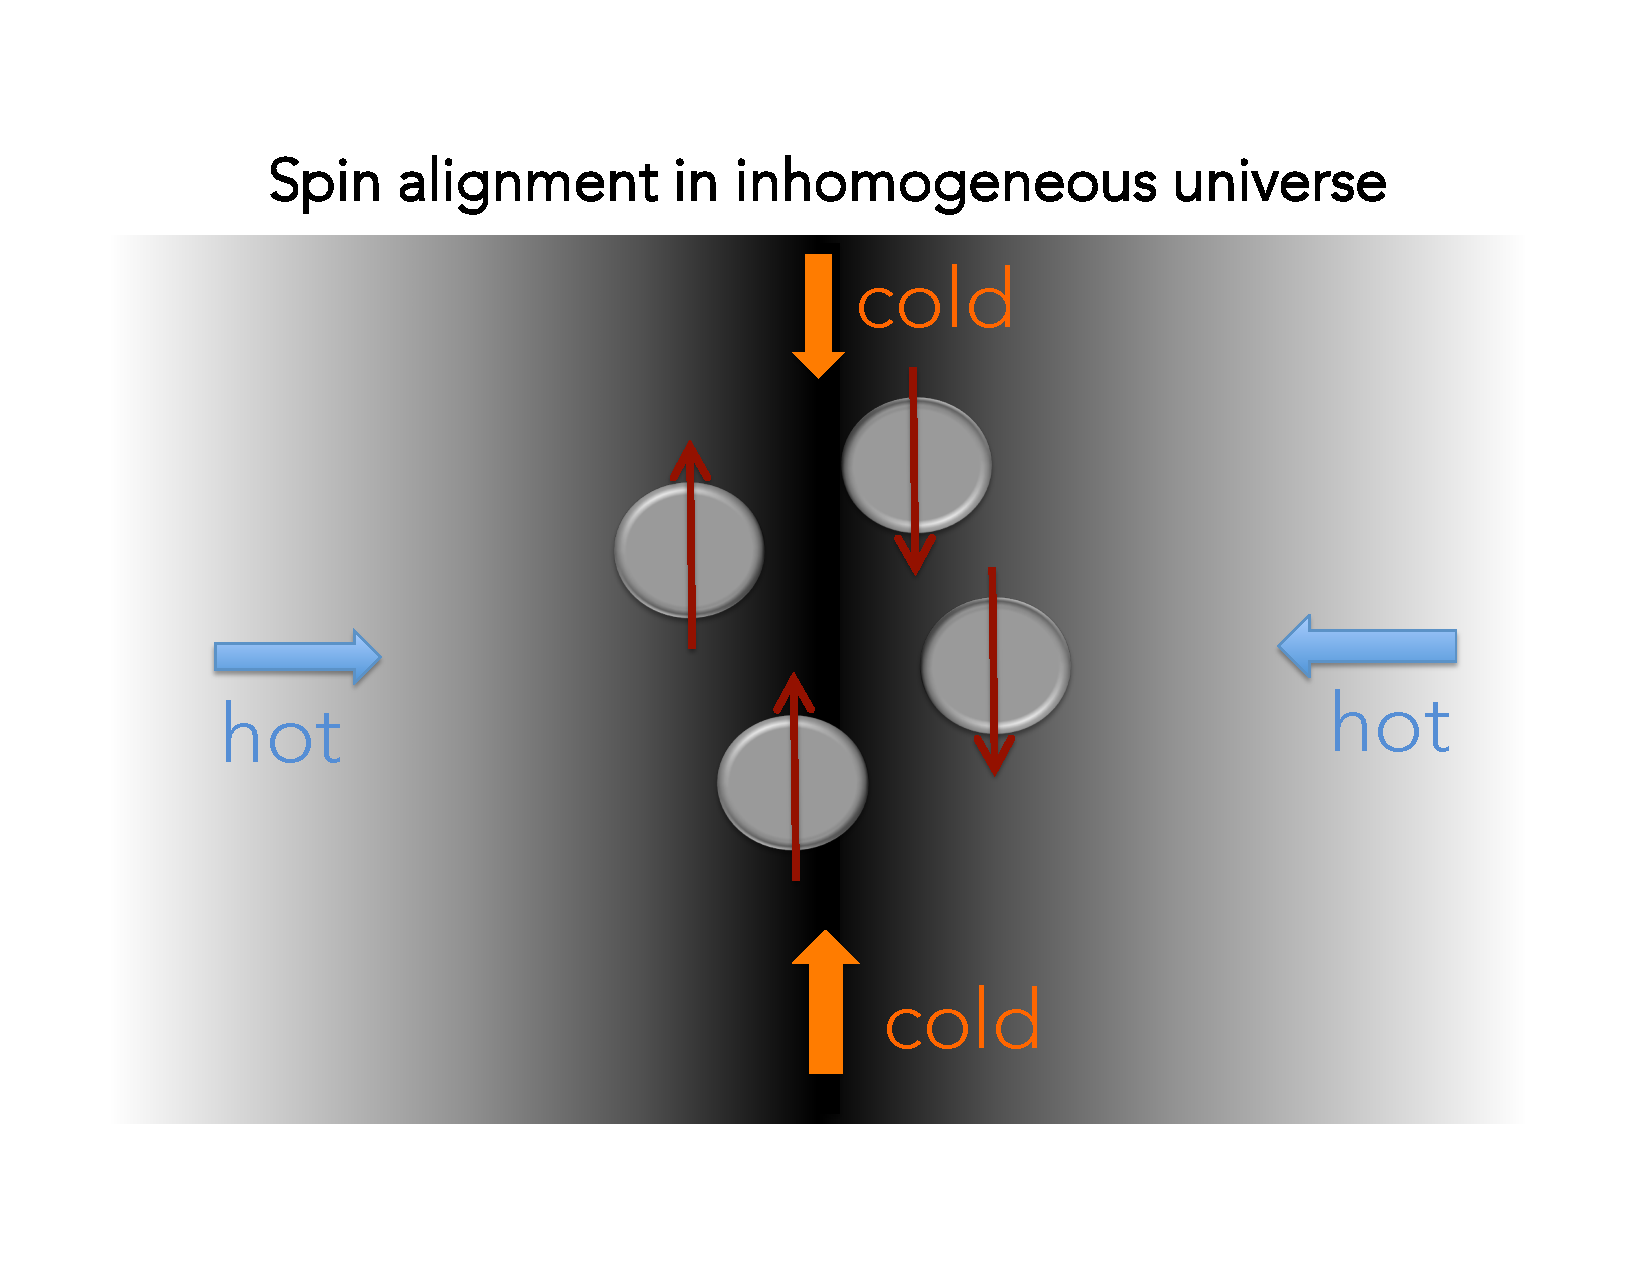
\includegraphics[width=.35\textwidth,keepaspectratio=true]{Slide2.pdf}
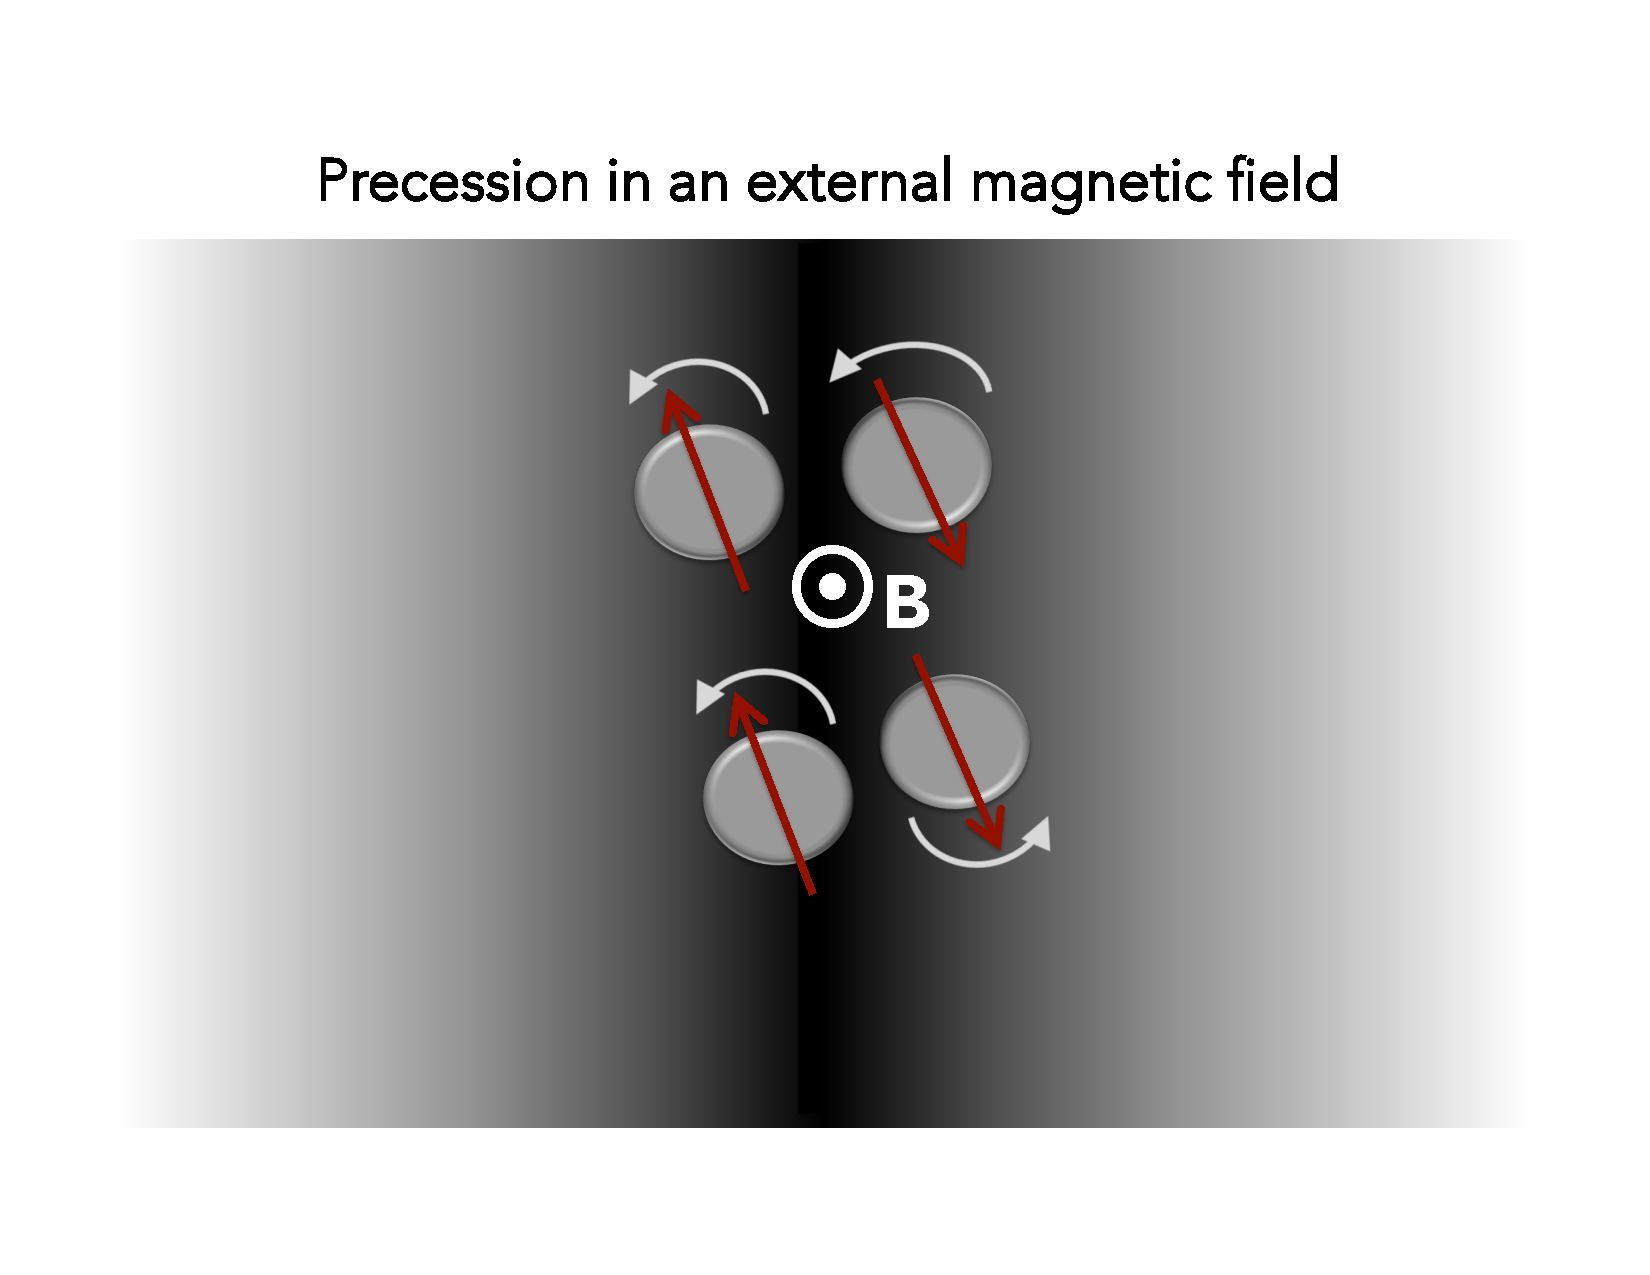
\includegraphics[width=.35\textwidth,keepaspectratio=true]{Slide3.pdf}
\caption{Illustration of the effect of a magnetic field on hydrogen atoms in the excited state of 21-cm transition at high redshifts. In the classical picture, magnetic moments of the atoms (depicted as red arrows) tend to be aligned with density gradients (upper panel; the gradient is depicted with the background shading), unless they precess about the direction of ambient magnetic field (pointing out of the page on the lower panel). When the precessing atoms decay back into the ground state, the emitted quadrupole (aligned with the direction of the magnetic moments) is misaligned with the incident quadrupole. This offset can be observed as a statistical anisotropy of 21-cm-brightness-temperature correlation functions, and used to trace cosmological magnetic fields.\label{fig:precession}}
\end{figure}
Magnetic moments of hydrogen atoms in the excited state of the 21-cm line transition tend to be aligned with the incident quadrupole of the 21-cm radiation from the surrounding medium. This effect of ``ground-state alignment'' \cite{Yan08,Yan12} arises in a cosmological setting due to velocity-field gradients. In the presence of external large-scale magnetic fields, the emitted 21-cm quadrupole is misaligned with the incident quadrupole, due to atomic precession (illustrated in Figure \ref{fig:precession}). The resulting emission anisotropy can thus be used to trace magnetic fields at high redshifts.

The main result of Paper I was a calculation of the 21-cm brightness temperature $T_{\rm b}$ as a function of the line of sight (LOS) direction ${\bf{\widehat n}}$, in the frame of the emitting ensamble of atoms. The relevant expression is
\beq
\bga
  \delta T_{\rm b}({\bf{\widehat n}}) = \left( 1 - \frac{T_\gamma}{T_{\rm s}} \right) x_{1{\rm s}} \left( \frac{1+z}{10} \right)^{1/2} \\
  \times \biggl[ 26.4 \ {\rm mK} \Bigl\{ 1 + \left(1 + ({\bf{\widehat k}} \cdot {\bf{\widehat n}})^2 \right)\delta \Bigr\}  
- 0.128 \ {\rm mK} \left( \frac{T_\gamma}{T_{\rm s}} \right)\\ \times x_{1{\rm s}} \left( \frac{1+z}{10} \right)^{1/2}  
 \Bigl\{ 1 + 2 \left(1 + ({\bf{\widehat k}} \cdot {\bf{\widehat n}})^2 \right)\delta \\
- \frac{ \delta }{15} \sum_m \frac{4\pi}{5} \frac{Y_{2 m}({\bf{\widehat k}}) \left[ Y_{2 m} ({\bf{\widehat n}}) \right]^* }{1 + x_{ \alpha, (2) } + x_{{\rm c}, (2)} - i m x_{\rm B}} \Bigr\} \biggr] \mbox{,} 
\ega
\label{eq:tbsoln}
\eeq
where $x_{\alpha, (2)}$, $x_{{\rm c}, (2)}$ and $x_{\rm B}$ parametrize the rates of depolarization of the ground state by optical pumping, collisions, and magnetic precession (relative to radiative depolarization), respectively (defined in detail in Paper I). Furthermore,  $T_{\rm s}$ and $T_\gamma$ are the spin temperature and the temperature of the cosmic microwave background at redshift $z$, respectively; $\bf{\widehat k}$ is a unit vector in the direction of the wave-vector $\vec k$ of a given density Fourier mode; and $Y_{2 m}$ represent the usual spin-zero spherical harmonics. Figure \ref{fig:hp} illustrates the effect of the magnetic field on the brightness temperature emission pattern in the frame of the atom; shown are quadrupole patterns corresponding to the sum-term of \eq{\ref{eq:tbsoln}}, for various strengths of the magnetic field. Notice that there is a saturation limit for the field strength---for strong enough fields, the precession time is much smaller than the lifetime in the excited state, and when the emission pattern assymptotes to the one shown in the bottom panel of Figure \ref{fig:hp}. Above this limit, approximation of linear dependence of $T_{\rm b}$ breaks down, which implies that the signal cannot be used to reconstruct the strength of the field; however, it is still possible to distinguish saturated regime from the case of null field, as we will see in \S\ref{sec:fisher}.
\begin{figure}
\centering
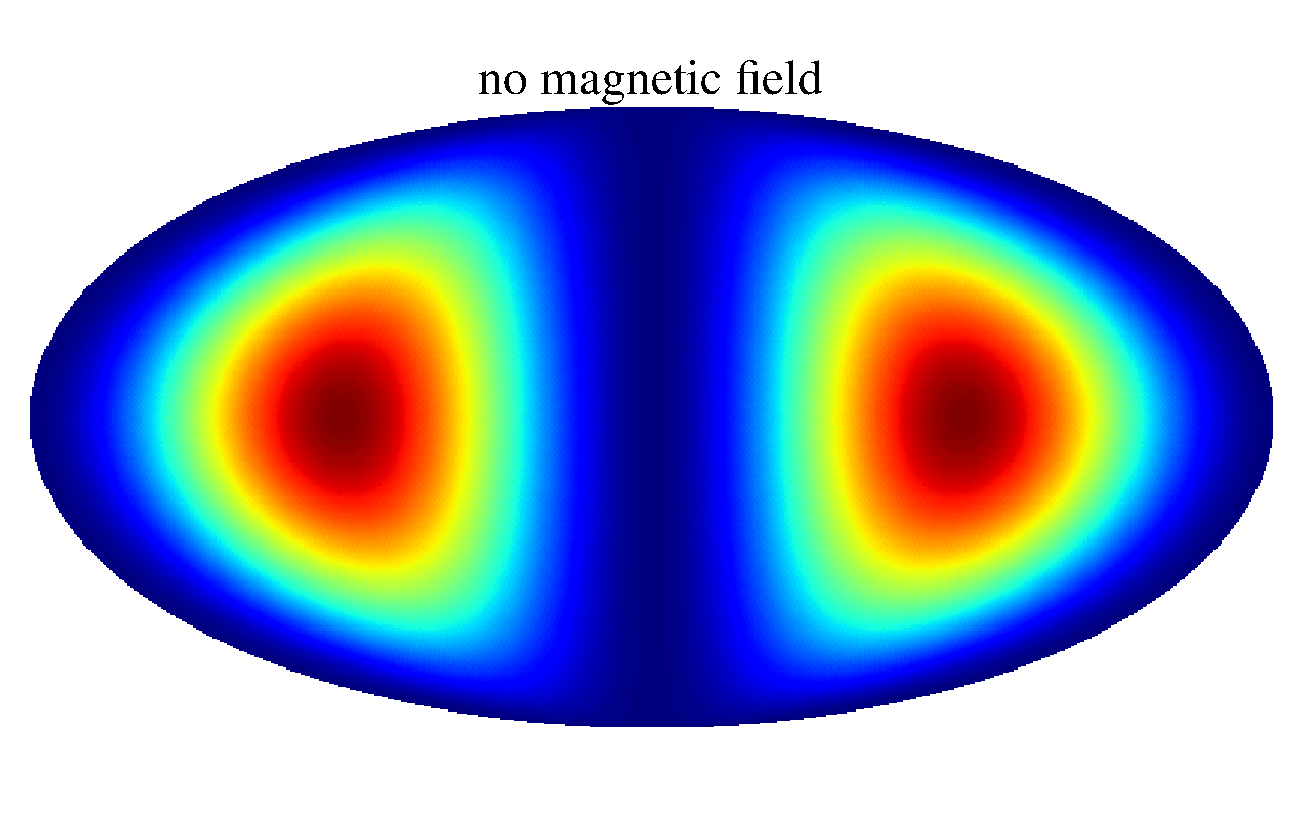
\includegraphics[width=.35\textwidth,keepaspectratio=true]{hp_B_0e+00G.pdf}
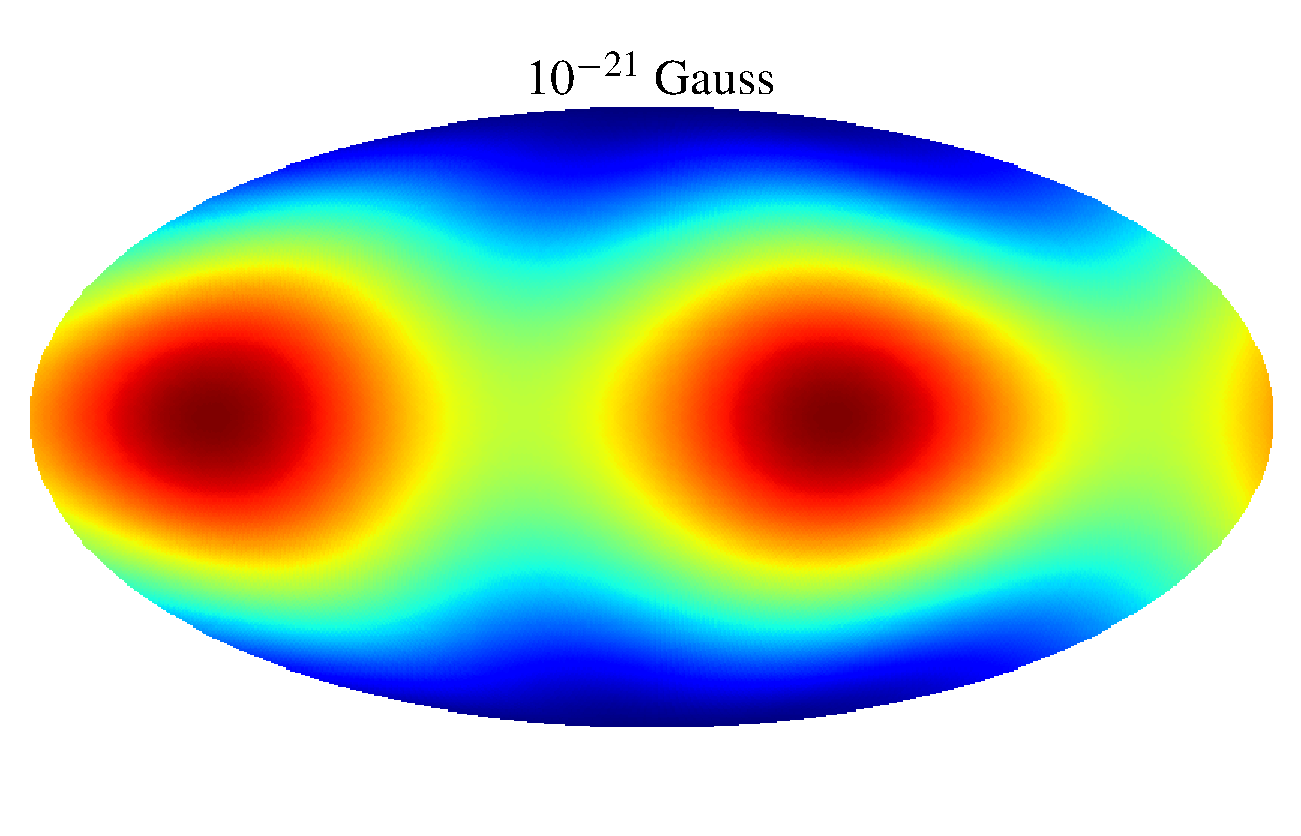
\includegraphics[width=.35\textwidth,keepaspectratio=true]{hp_B_1e-18G.pdf}
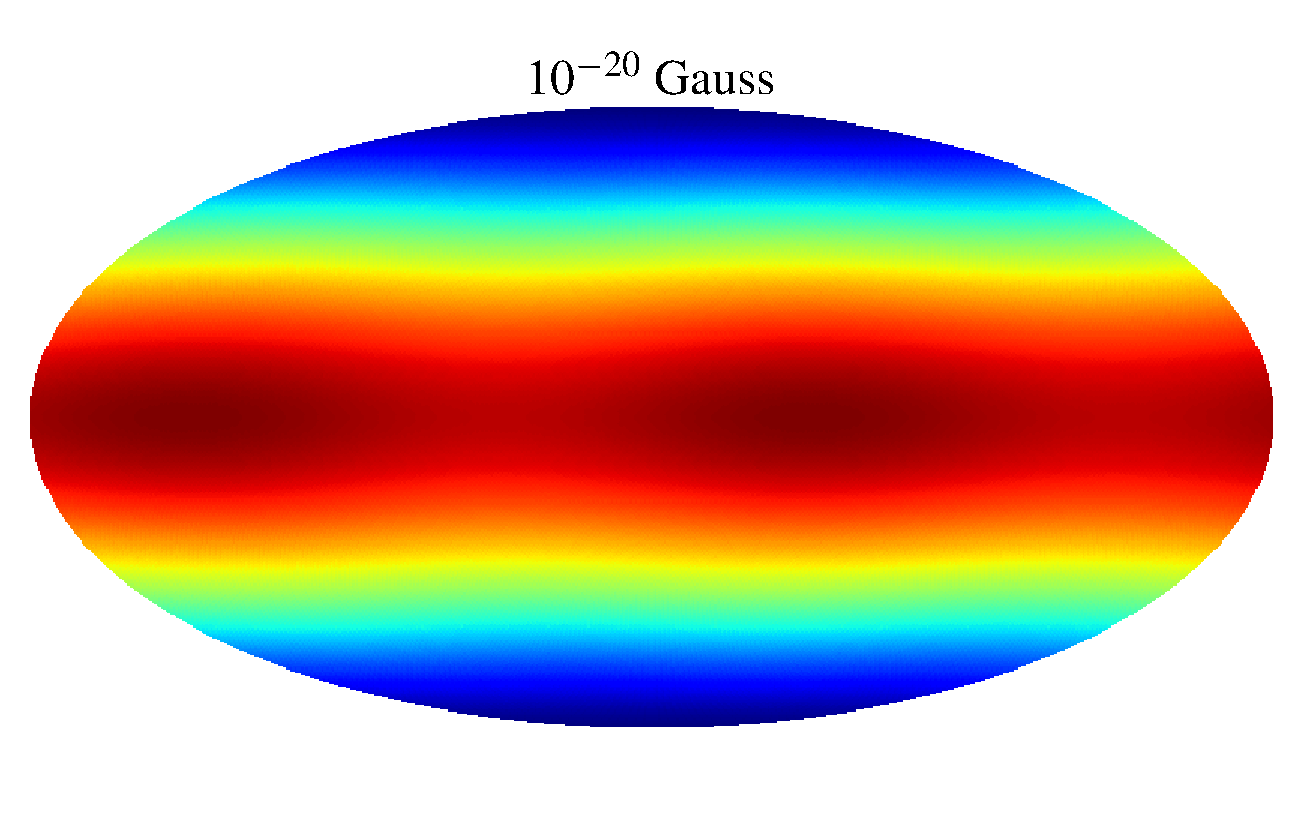
\includegraphics[width=.35\textwidth,keepaspectratio=true]{hp_B_1e-17G.pdf}
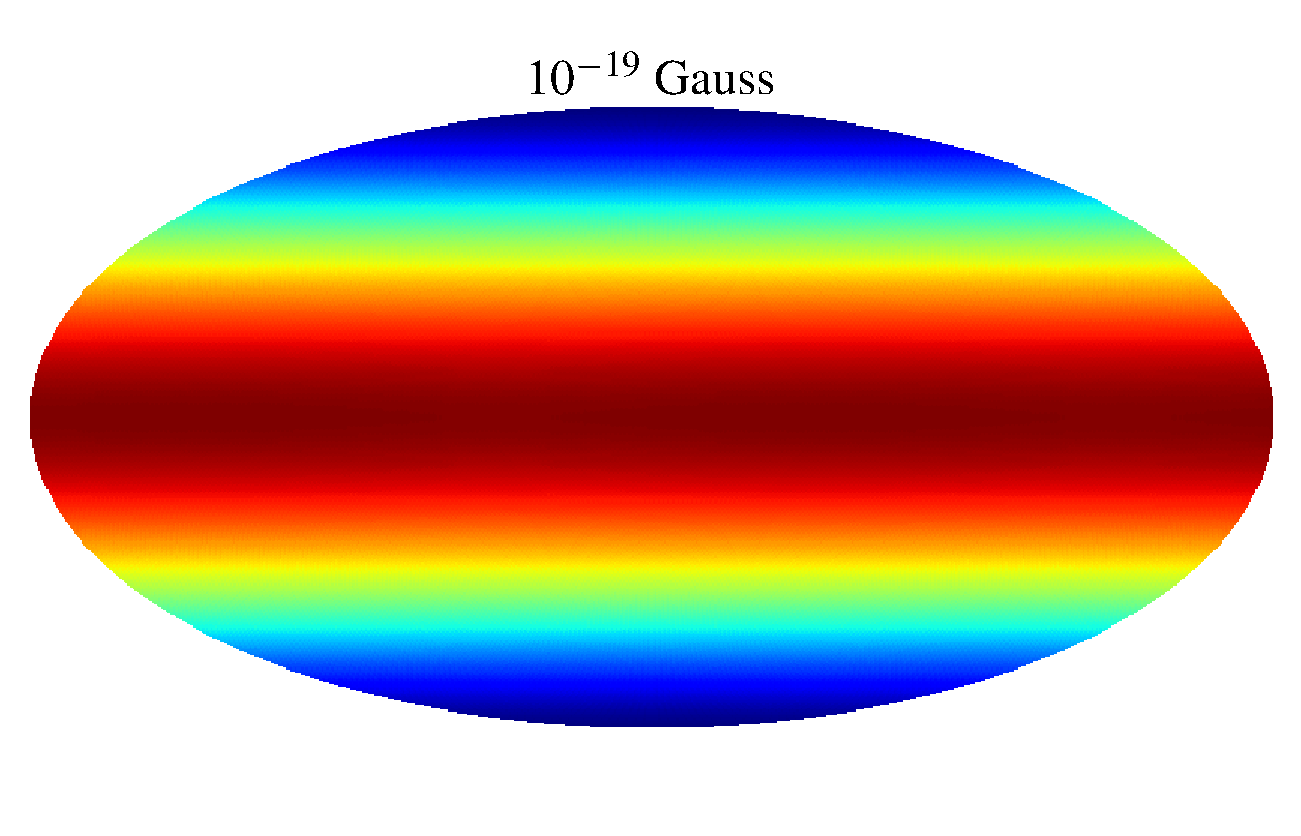
\includegraphics[width=.35\textwidth,keepaspectratio=true]{hp_B_1e-16G.pdf}
\caption{Illustration of the quadrupolar pattern of 21-cm emission from the last ($B$-dependent) term of \eq{\ref{eq:tbsoln}} in the frame of the emitting atoms, for the case where $\vec k$ is perpendicular to ${\bf{\widehat n}}$ (maximal signal), shown in Molleweide projection. Lower panels correspond to increasingly stronger magnetic fields (strength denoted on each panel in comoving units), with the bottom panel corresponding to the saturated case. Notice how the type of quadrupole differs for the no-magnetic field case and the case the field is ``strong'' in the saturation sense. \label{fig:hp}}
\end{figure}

The affect of quadrupole misalignement arises at second order in optical depth (it is a result of a two-scattering process), and is thus a small correction to the total brightness temperature. However, owing to the long lifetime of the excited state (during which even an extremely slow precession has large cumulative effect on the direction of the quadrupole at second order), the effect of misalignement is excuisitively sensitive to magnetic fields in the IGM at redshifts prior to cosmic reionization---as we show in Paper I, a miniscule magnetic field strength of  $10^{-21}$ Gauss (in comoving units) produces order-one changes in the direction of the quadrupole. This means that a high-precision measurement of the 21-cm brightness-temperature 2-point correlation function intrinsically has that level of sensitivity to detecting magnetic fields in the Dark Ages. We now proceed to develop a formalism to search for this effect, with future surveys of redshifted 21-cm line, and to identifying experimental setups that can reach it. 